\section{Case Study: Key-Value Store}
\label{sec:kvs}
The next two sections contain case studies that show how \lang can be used to
build practical distributed programs. Both case studies are monotonic programs:
that is, both programs consist of monotone functions applied to lattices. This
ensures that the values computed by the programs ``grow'' over time---these
examples show the various kinds of forward progress that can be encoded using
\lang.

In the first case study, we show that a distributed key-value store (KVS) can be
\emph{composed} via a series of monotonic mappings between simple lattices. By
composing a complex program from simple lattices, we show that \lang's built-in
lattices are useful; morever, the resulting KVS implementation is concise,
readable, and has clear semantics.

%  This
% demonstrates that \lang's built-in lattices are useful and yields a very concise
% implementation. Morever, using lattice composition gave us confidence in the
% correctness of our code, because much of the program's complexity resides in
% simple built-in lattices that we 

%  More importantly, composing a complex program from simple
% lattices made it easy to reason about the behavior of the entire program

%  and results in a very
% concise implementation. Moreover, it gives us confidence in the correctness of
% our implementation, because much of the program's complexity is handled by the
% behavior of the built-in lattices, which are likely to be correct.  \paa{not
%   sure what to suggest, but this last clause seems underconfident (and slightly
%   run-on).  perhaps we just want to say that we assert them to be correct, or
%   that it's easy to prove/convince ourselves that they are correct due to their
%   simplicity, etc}

\subsection{Basic Architecture}
\begin{figure}[t]
\begin{scriptsize}
\begin{lstlisting}
module KvsProtocol
  state do
    channel :kvput, [:reqid, :@addr] => [:key, :val,
                                         :client_addr]
    channel :kvput_resp, [:reqid] => [:@addr, :replica_addr]
    channel :kvget, [:reqid, :@addr] => [:key, :client_addr]
    channel :kvget_resp, [:reqid] => [:@addr, :val,
                                      :replica_addr]
  end
end
\end{lstlisting}
\end{scriptsize}
\caption{Key-value store interface.}
\label{fig:kvs-interface}
\end{figure}

\begin{figure}[t]
\begin{scriptsize}
\begin{lstlisting}
class KvsReplica
  include Bud
  include KvsProtocol

  state { lmap :kv_store } (*\label{line:kvs-map-ddl}*)

  bloom do
    kv_store   <= kvput {|c| {c.key => c.val}} (*\label{line:kvs-put-merge}*)
    kvput_resp <~ kvput {|c| [c.reqid, c.client_addr, ip_port]}
    kvget_resp <~ kvget {|c| [c.reqid, c.client_addr,
                              kv_store.at(c.key), ip_port]}
  end
end
\end{lstlisting}
\end{scriptsize}
\caption{KVS replica implementation in \lang.}
\label{fig:kvs-replica}
\end{figure}

% duplicate introduction of KVS acronym -- remove?
A key-value store (KVS) provides a lookup service that allows client
applications to retrieve the \emph{value} associated with a given \emph{key}. In
a typical KVS, key-value pairs are replicated on multiple server replicas for
redundancy and the keyspace is partitioned in some fashion to improve aggregate
storage and throughput. \emph{Eventual consistency} is a common correctness
criterion: after all client updates have reached all storage nodes, all the
replicas of a key-value pair will converge to the same final
state~\cite{Terry1995,vogels}.

Figure~\ref{fig:kvs-interface} shows a simple KVS interface in \lang. Client
applications submit \emph{get(key)} and \emph{put(key, val)} operations by
inserting into the \texttt{kvget} and \texttt{kvput} channels, respectively;
server replicas return responses via the \texttt{kvget\_resp} and
\texttt{kvput\_resp} channels.

Figure~\ref{fig:kvs-replica} contains the \lang code for a KVS server
replica. An \texttt{lmap} lattice is used to maintain the mapping between keys
and values (line~\ref{line:kvs-map-ddl}). Since the values in an \texttt{lmap}
lattice must themselves be lattice elements, for now we assume that clients only
want to store and retrieve lattice values; we discuss how to support arbitrary
values in Section~\ref{sec:kvs-versions}. To handle a \emph{put(key, val)}
request, a new \emph{key} $\to$ \emph{val} \texttt{lmap} is created and merged
into \texttt{kv\_store} (line~\ref{line:kvs-put-merge}). If \texttt{kv\_store}
already contains a value for the given key, the two values will be merged
together using the value lattice's merge function (see
Section~\ref{sec:lattice-built-ins} for details). Note that we use the \lang
features described in Section~\ref{sec:bloom-interop} to allow traditional Bloom
collections (e.g., channels) and lattices (e.g., the \texttt{kv\_store} lattice)
to be used by the same program. Note also that \texttt{ip\_port} is a built-in
function that returns the IP address and port number of the current Bud
instance.

The state of two replicas can be synchronized by simply exchanging their
\texttt{kv\_store} maps; the \texttt{lmap} merge function will automatically
resolve all conflicting updates made to the same key. This property allows
considerable flexibility in how replicas propagate updates.
% TODO: (1) finish repl discussion (composition, replication strat) (2) partitioning

\subsection{Object Versioning}
\label{sec:kvs-versions}
\begin{figure}[t]
\centering
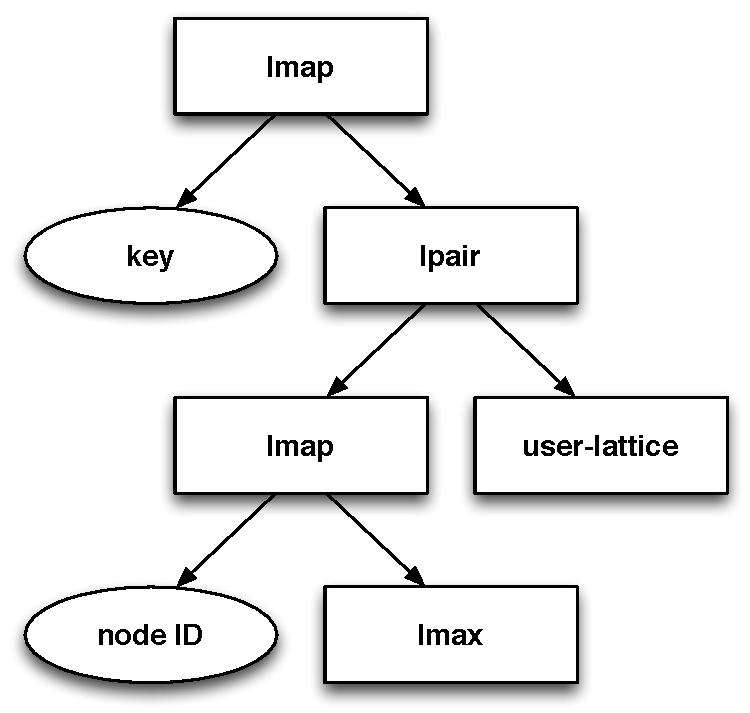
\includegraphics[width=0.8\linewidth]{fig/kvs-vc-lattice.pdf}
\caption{Lattice structure of a KVS with object versioning. Rectangles are
  lattices and ovals are atomic values.}
\label{fig:kvs-vc-lattices}
\end{figure}

The basic KVS design is sufficient for applications that want to store
monotonically increasing values, such as session logs or increasing counters. To
allow storage of values that change in arbitrary ways, we now consider how to
support \emph{object versions}. This is a classic technique for recognizing
mutual inconsistency between members of a distributed system~\cite{Parker1983};
our design is similar to that used by Dynamo~\cite{DeCandia2007}.

Each replica associates keys with
$\langle\textit{vector-clock},\textit{value}\rangle$ pairs. The vector clock
(VC) captures the causal relationship between different versions of a
record~\cite{Fidge1988,DeCandia2007}. Clients get and put
$\langle\textit{vector-clock},\textit{value}\rangle$ pairs. When a client
updates a value it has previously read, the client increments its own position
in the VC and includes the updated vector clock $V_U$ with its \emph{put}
operation. Upon receiving an update, the server compares $V_U$ with the VC of
the server's version of the record ($V_S$). If $V_U > V_S$, the server replaces
the stored record with the client's update. If $V_S > V_U$, the update is
ignored (this situation might arise due to duplication and reordering of
messages by the network). If $V_U$ and $V_S$ are incomparable, the two versions
are concurrent, so a client-supplied reconciliation function is used to resolve
the conflict.

From a \lang perspective, each replica still stores a monotonically increasing
value---the only difference is that in this scheme, the \emph{version} stored by
a replica increases over time, rather than the associated value. Hence, we now
consider how to support vector clocks and version-value pairs using \lang.

\subsubsection{Vector Clocks}
\nrc{Ugh, TODO.}
Vector clocks are a well-known mechanism for recording the causal relationships
between events~\cite{Fidge1988}. A vector clock is a map from node identifiers
to logical clocks. Each event $e$ is associated with a vector clock $V_e$; if
$V_e < V_{e'}$, $e$ causally precedes $e'$.

In \lang, a vector clock can be represented as an \texttt{lmap} that maps node
identifiers to \texttt{lmax} values. \texttt{lmax} is appropriate, since the
logical clock value associated with a given node will only increase over
time. The merge function provided by \texttt{lmap} achieves the desired
semantics.

\subsubsection{Version-Value Pairs}
We now turn to representing $\langle\textit{vector-clock},\textit{value}\rangle$
pairs. To do this, we define a new lattice \texttt{lpair} that ``wraps'' two
lattice elements; we use \emph{fst} and \emph{snd} to refer to the first and
second elements of an \texttt{lpair}, respectively. The discussion above
suggests a natural least upper bound for \texttt{lpair}:
\begin{displaymath}
  A \sqcup B = \left\{
    \begin{array}{l l}
      A & \textrm{if } A.\textit{fst} > B.\textit{fst} \\
      B & \textrm{if } A.\textit{fst} < B.\textit{fst} \\
      \langle A.\textit{fst} \sqcup B.\textit{fst}, A.\textit{snd} \sqcup B.\textit{snd}\rangle & \textrm{otherwise} \\
    \end{array} \right. 
\end{displaymath}
This implements the desired semantics: given two candidate values for a key, the
candidate with the strictly greater version number should be preferred. When the
two versions are incomparable, a new \texttt{lpair} should be formed by merging
both elements of the input pairs with one another. In the case of the KVS,
\emph{fst} is a vector clock, while \emph{snd} is the user's data; the least
upper bound of the \emph{snd} lattice corresponds to a user-defined merge
function.\footnote{If the user stores a value that does not have a merge
  function, similar systems typically provide a default merge function that
  collects conflicting updates for eventual manual resolution by the user. Such
  a strategy could easily be implemented with \lang.}

Note that while the \emph{fst} of a given \texttt{lpair} increases over time (as
new versions are received), the \emph{snd} may not (a newer version might
contain a ``smaller'' \emph{snd}). Again, this is the desired behavior.

\subsubsection{Discussion}
Figure~\ref{fig:kvs-vc-lattices} shows the lattices used in the KVS with object
versioning. Surprisingly, adding support for object versioning did not require
\emph{any} changes to the KVS replica code! Instead, clients simply store
\texttt{lpair} values containing a vector clock as the first element and
increment their position in the vector clock when submitting updates. The KVS
replica merges these \texttt{lpair} values into an \texttt{lmap} as usual; the
merge function of \texttt{lpair} handles conflict resolution in the appropriate
manner. Moreover, by composing the KVS from a collection of simple lattices, we
found it easy to reason about the behavior of the system. For example,
convincing ourselves that the KVS replicas will eventually converge only
required checking that the individual \texttt{lmap}, \texttt{lmax}, and
\texttt{lpair} lattices satisfy the lattice properties, rather than analyzing
the behavior of the system as a whole.

Our design compares favorably to traditional implementations of object
versioning and vector clocks. For example, the implementation of vector clocks
in Voldemort (a popular key-value store) requires 216 lines of Java, not
including whitespace or comments~\cite{voldemort-vector-clock}. In \lang, vector
clocks follow directly from the composition of the \texttt{lmap} and
\texttt{lmax} lattices; the entire KVS requires only 53 lines of Ruby and \lang
code, including the client library. The \texttt{lpair} lattice required 30 lines
of Ruby but is completely generic, and would be suitable for inclusion as a
built-in lattice.

\subsection{Quorum Reads and Writes}
A common KVS feature is the ability to submit reads and writes to a configurable
number of nodes. If a client reads from $R$ nodes and writes to $W$ nodes in a
KVS with $N$ replicas, the user can set $R + W > N$ to achieve behavior
equivalent to a quorum replication system~\cite{Gifford1979}, or use smaller
values of $R$ and $W$ if eventual consistency is sufficient. This scheme allows
users to vary $R$ and $W$ on a per-operation basis, depending on their
consistency and durability requirements.

To support this feature, we can use the \lang quorum voting pattern first
introduced in Figure~\ref{fig:lattice-quorum}. After sending a write to $W$
systems, the KVS client accumulates \texttt{kvput\_resp} messages into an
\texttt{lset}. Testing for quorum can be done in a monotonic fashion by mapping
the \texttt{lset} to an \texttt{lmax} (using the \texttt{size} method), and then
performing a threshold test using \texttt{gt\_eq} on \texttt{lmax}. As expected,
this is monotonic: once quorum has been reached, it will never be retracted.

Quorum reads work in a similar fashion, except that the client must also merge
together the $R$ versions of the record it receives. This follows naturally from
the discussion in Section~\ref{sec:kvs-versions}: the client simply takes the
least upper bound of the values it receives, which produces the expected
behavior. The client can optionally write the merged value back to the KVS
(so-called ``read repair''~\cite{DeCandia2007}); note that the \texttt{lpair}
merge method also updates the record's vector clock appropriately.
